\documentclass{article}
\usepackage{geometry}
\geometry{
	a4paper,
	left=2.5cm,
	right=2.5cm,
	top=2.5cm,
	bottom=2.5cm,
	headheight=13.6pt
}

\usepackage{fontspec}
\usepackage{ctex}

\setmainfont{Times New Roman}[
BoldFont = Times New Roman Bold,
ItalicFont = Times New Roman Italic,
BoldItalicFont = Times New Roman Bold Italic
]

\setCJKmainfont{SimSun}[
BoldFont = SimHei,
ItalicFont = KaiTi
]

\usepackage{amsmath}
\usepackage{booktabs}
\usepackage{caption}
\usepackage{setspace}
\usepackage{array}
\usepackage{graphicx}
\usepackage{enumitem}
\usepackage{subcaption}
\usepackage{multirow}

\captionsetup[table]{
	justification=centering,
	labelsep=quad,
	font={bf,small}
}
\captionsetup[figure]{
	justification=centering,
	labelsep=quad,
	font={bf,small}
}

\begin{document}
	
	\begin{center}
		{\LARGE \textbf{中学数学建模试题}} \\[0.5cm]
		{\large 石继楷 \quad 202411079123} \\[0.3cm]
		{\large 2026年5月13日}
	\end{center}
	
	激光位移传感器是一种利用激光三角测量法或光飞行时间法来测量工件表面轮廓的非接触式测量设备。传感器将激光束投射到被测工件表面，通过接收反射光计算传感器到表面的距离。当传感器沿直线导轨移动时，能够获得一条连续的表面轮廓线，但单次扫描只能获取一条线上的数据，无法同时获得垂直于运动方向的表面信息。
	
	\begin{figure}[h!]
		\centering
		\subcaptionbox{单点激光测量原理\label{fig:图1a}}
		{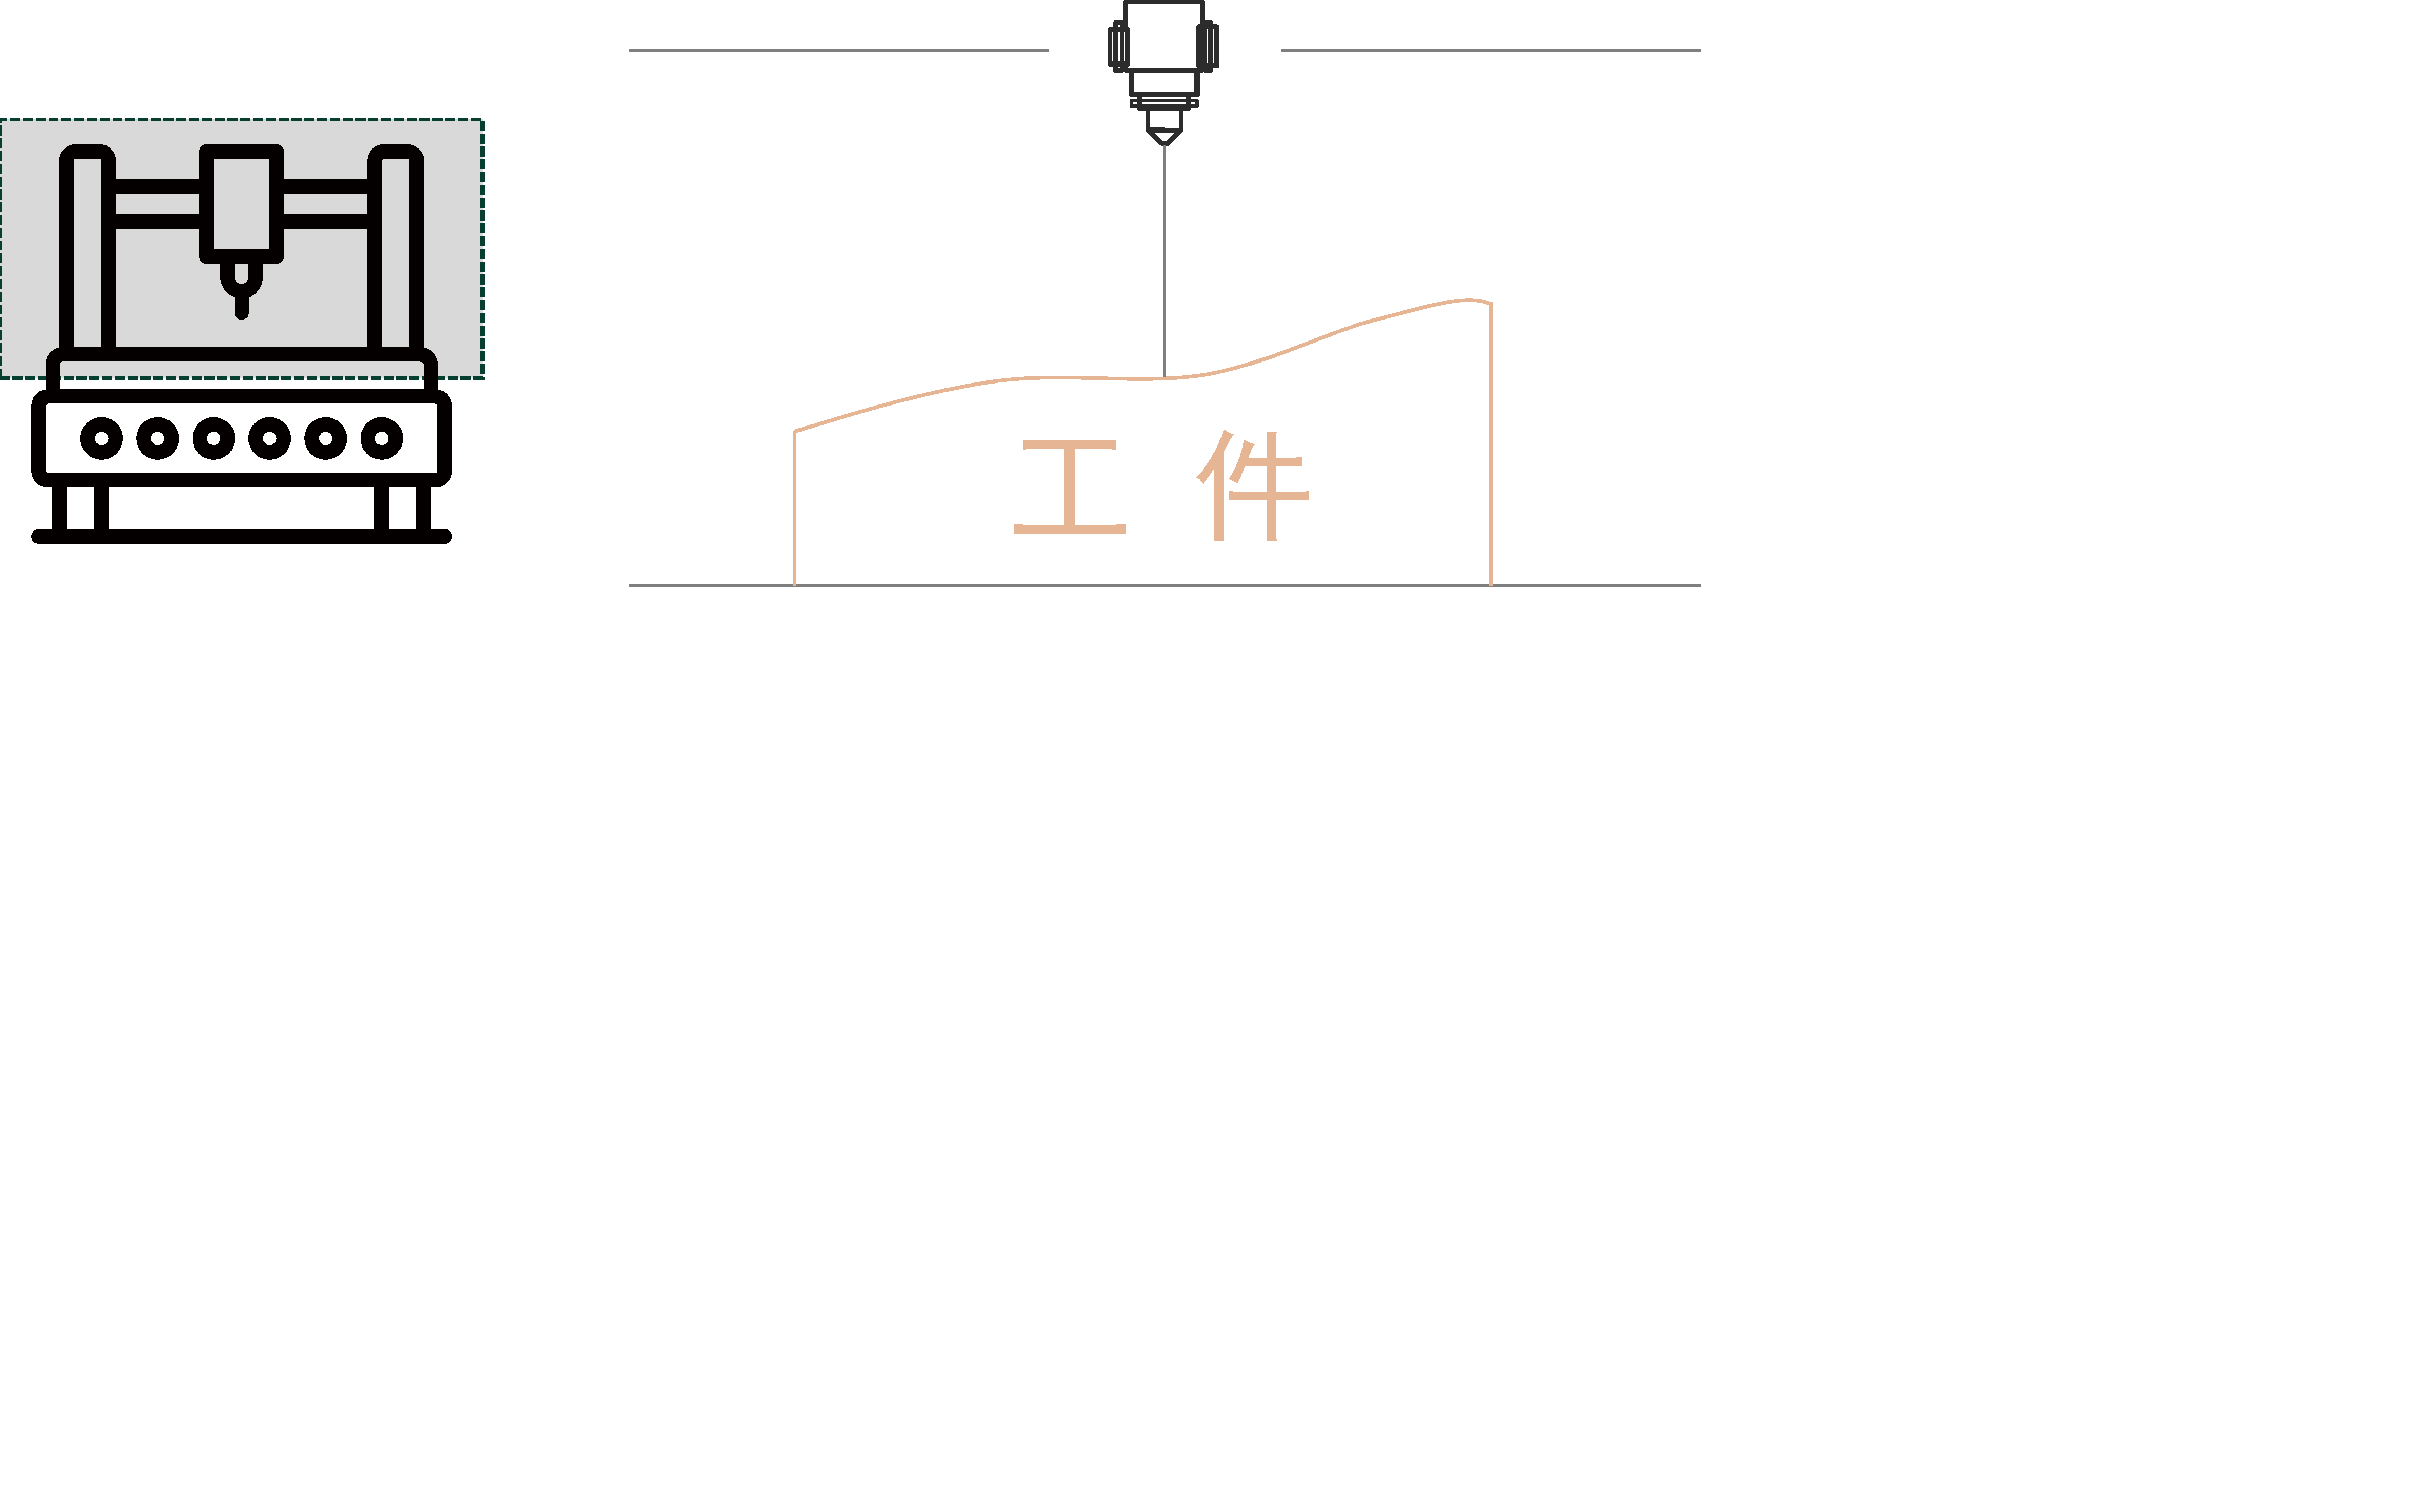
\includegraphics[width=0.5\textwidth,trim=0cm 30cm 22cm 0cm,clip]{figures/图1.pdf}}
		\subcaptionbox{线激光测量原理\label{fig:图1b}}
		{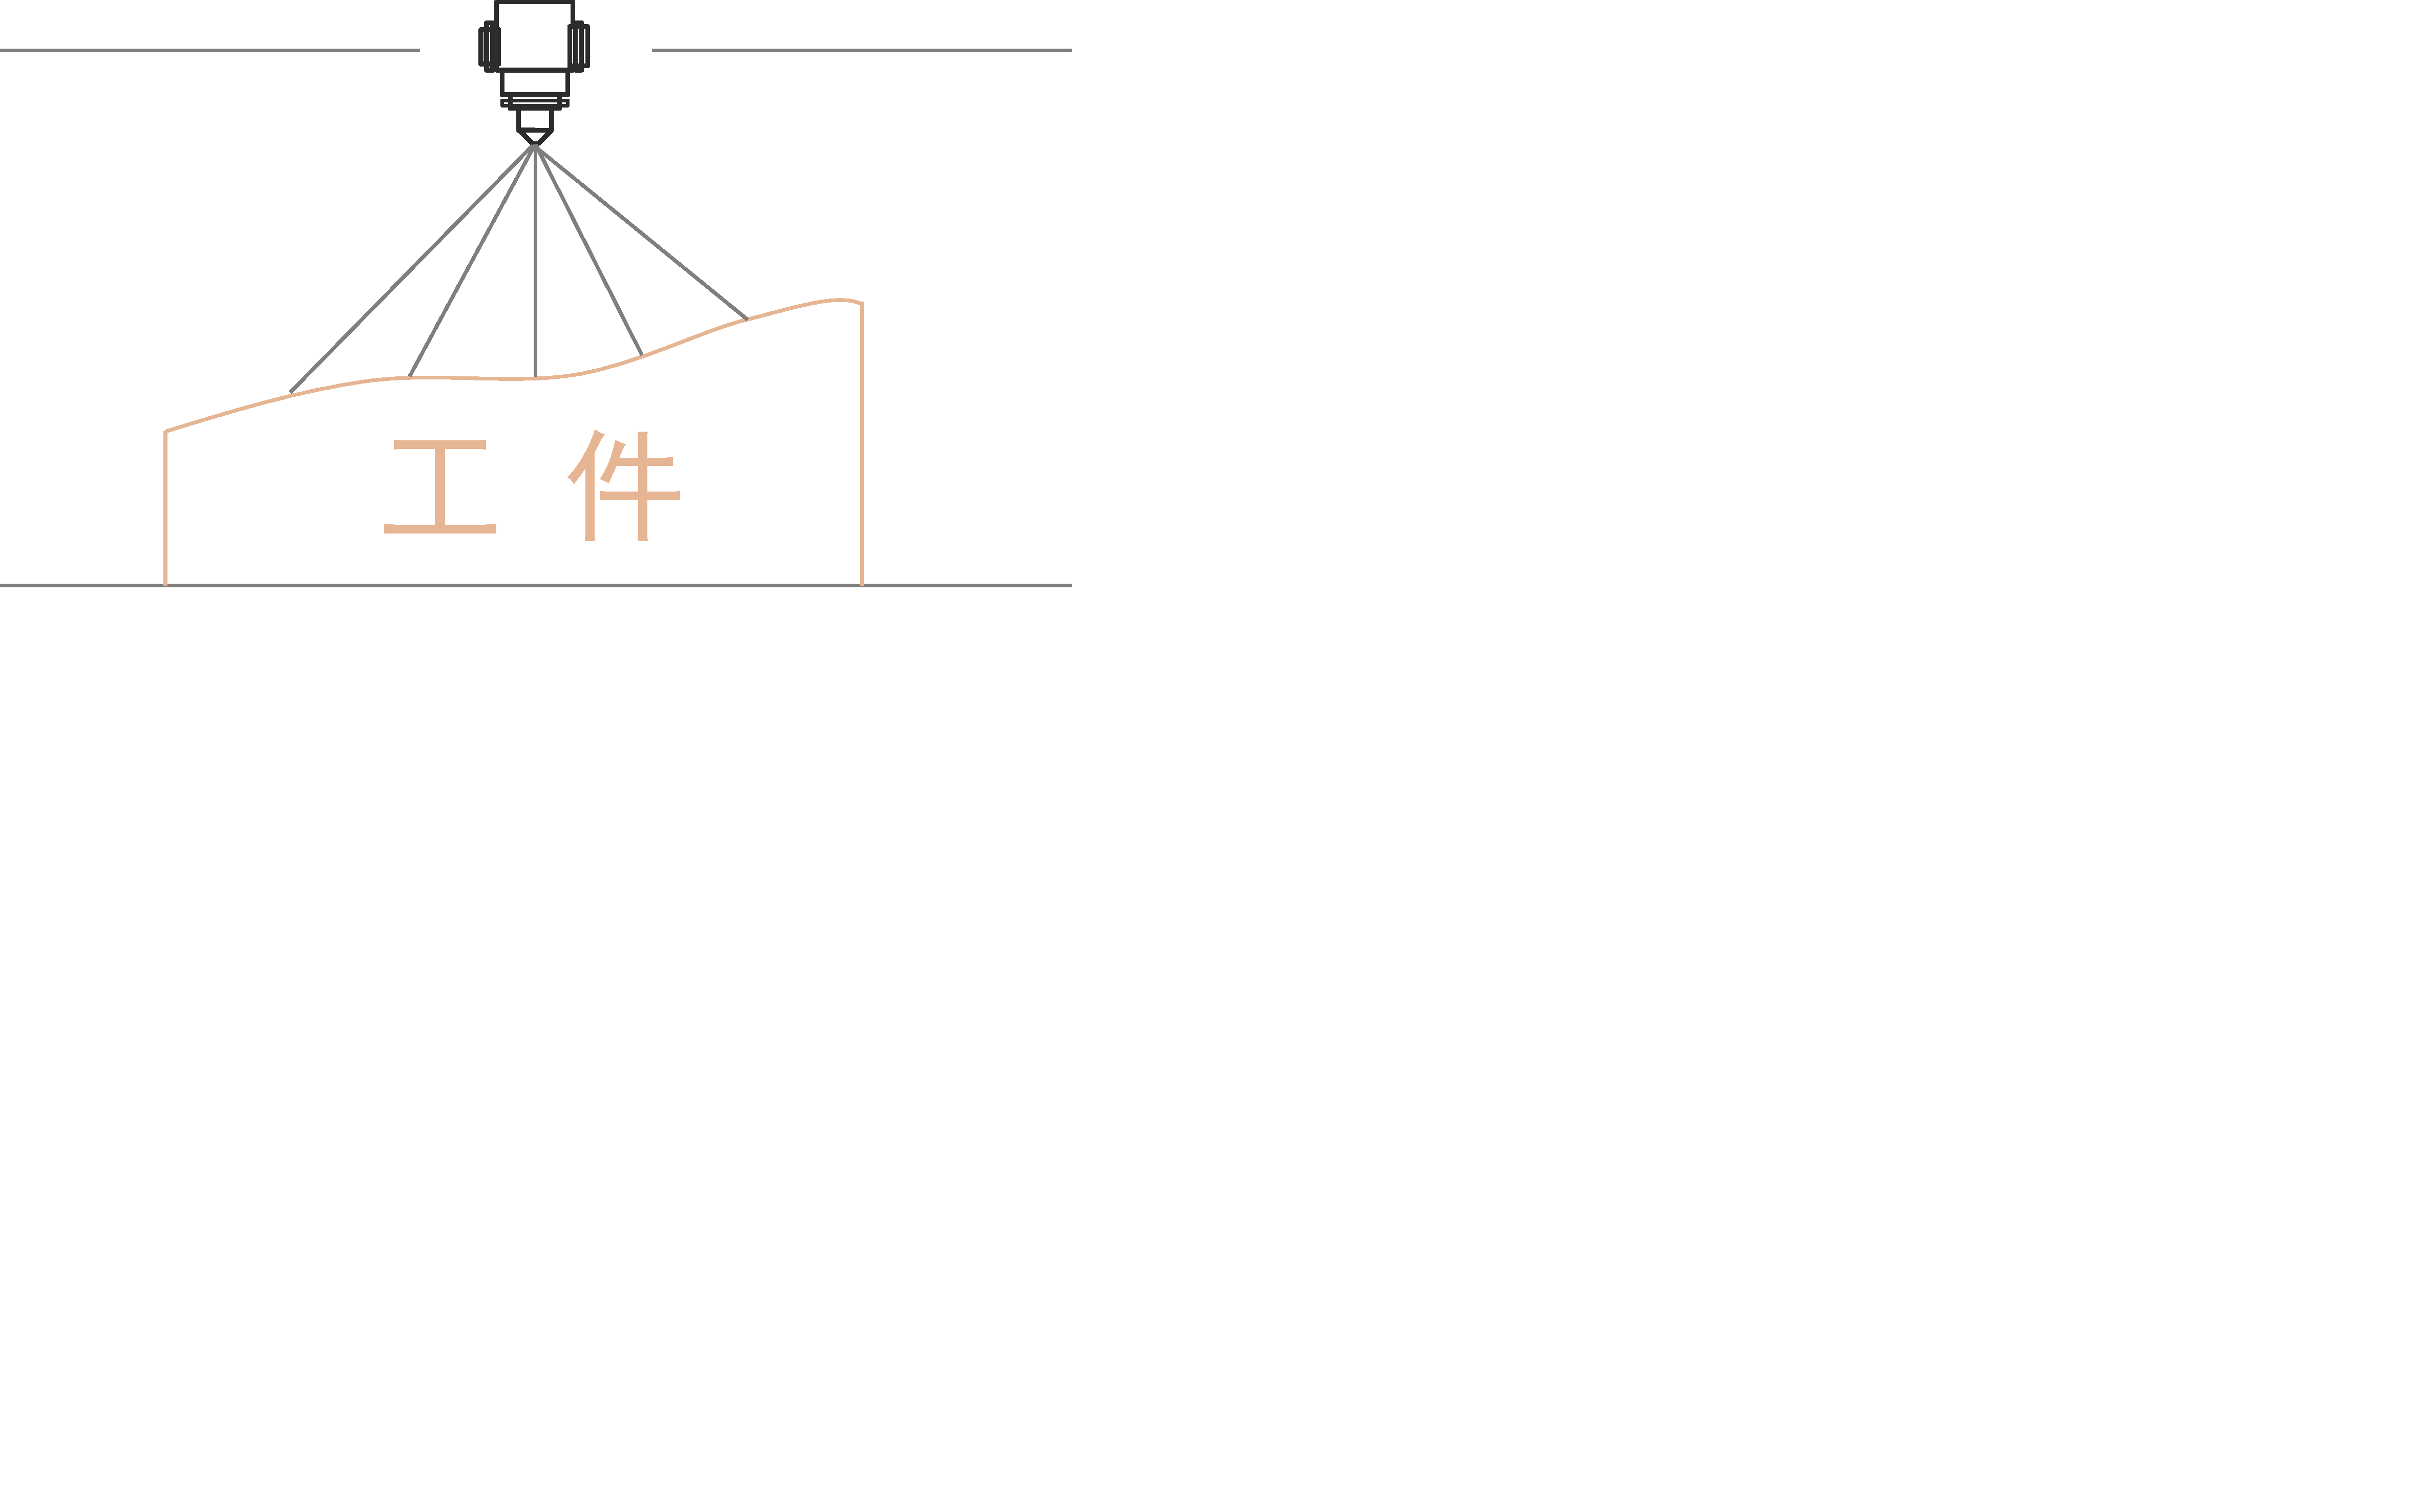
\includegraphics[width=0.3\textwidth,trim=0cm 30cm 45cm 0cm,clip]{figures/图2.pdf}}
		\caption{单点激光与线激光测量原理}
		\label{fig:波束对比}
	\end{figure}
	
	线激光测量系统是在单点激光测量的基础上发展起来的，该系统在垂直于导轨方向的平面内一次能投射出多条激光线，由相机接收经工件表面漫反射的激光，其工作原理如图\ref{fig:图1b}所示。线激光测量系统克服了单点测量的缺点，能够获得以导轨方向为轴线、具有一定宽度的全覆盖轮廓数据。
	
	线激光测量的覆盖宽度 \(W\) 随激光发射张角 \(\theta\) 和测量距离 \(D\) 的变化而变化。若扫描路径相互平行且工件表面平行于水平面，则相邻扫描条带之间的重叠率定义为 \(\eta = 1 - \frac{d}{W}\)，其中 \(d\) 为相邻两条扫描路径的间距，\(W\) 为条带的覆盖宽度。
	
	\begin{figure}[h!]
		\centering
		\subcaptionbox{扫描条带及重叠区域\label{fig:图2a}}
		{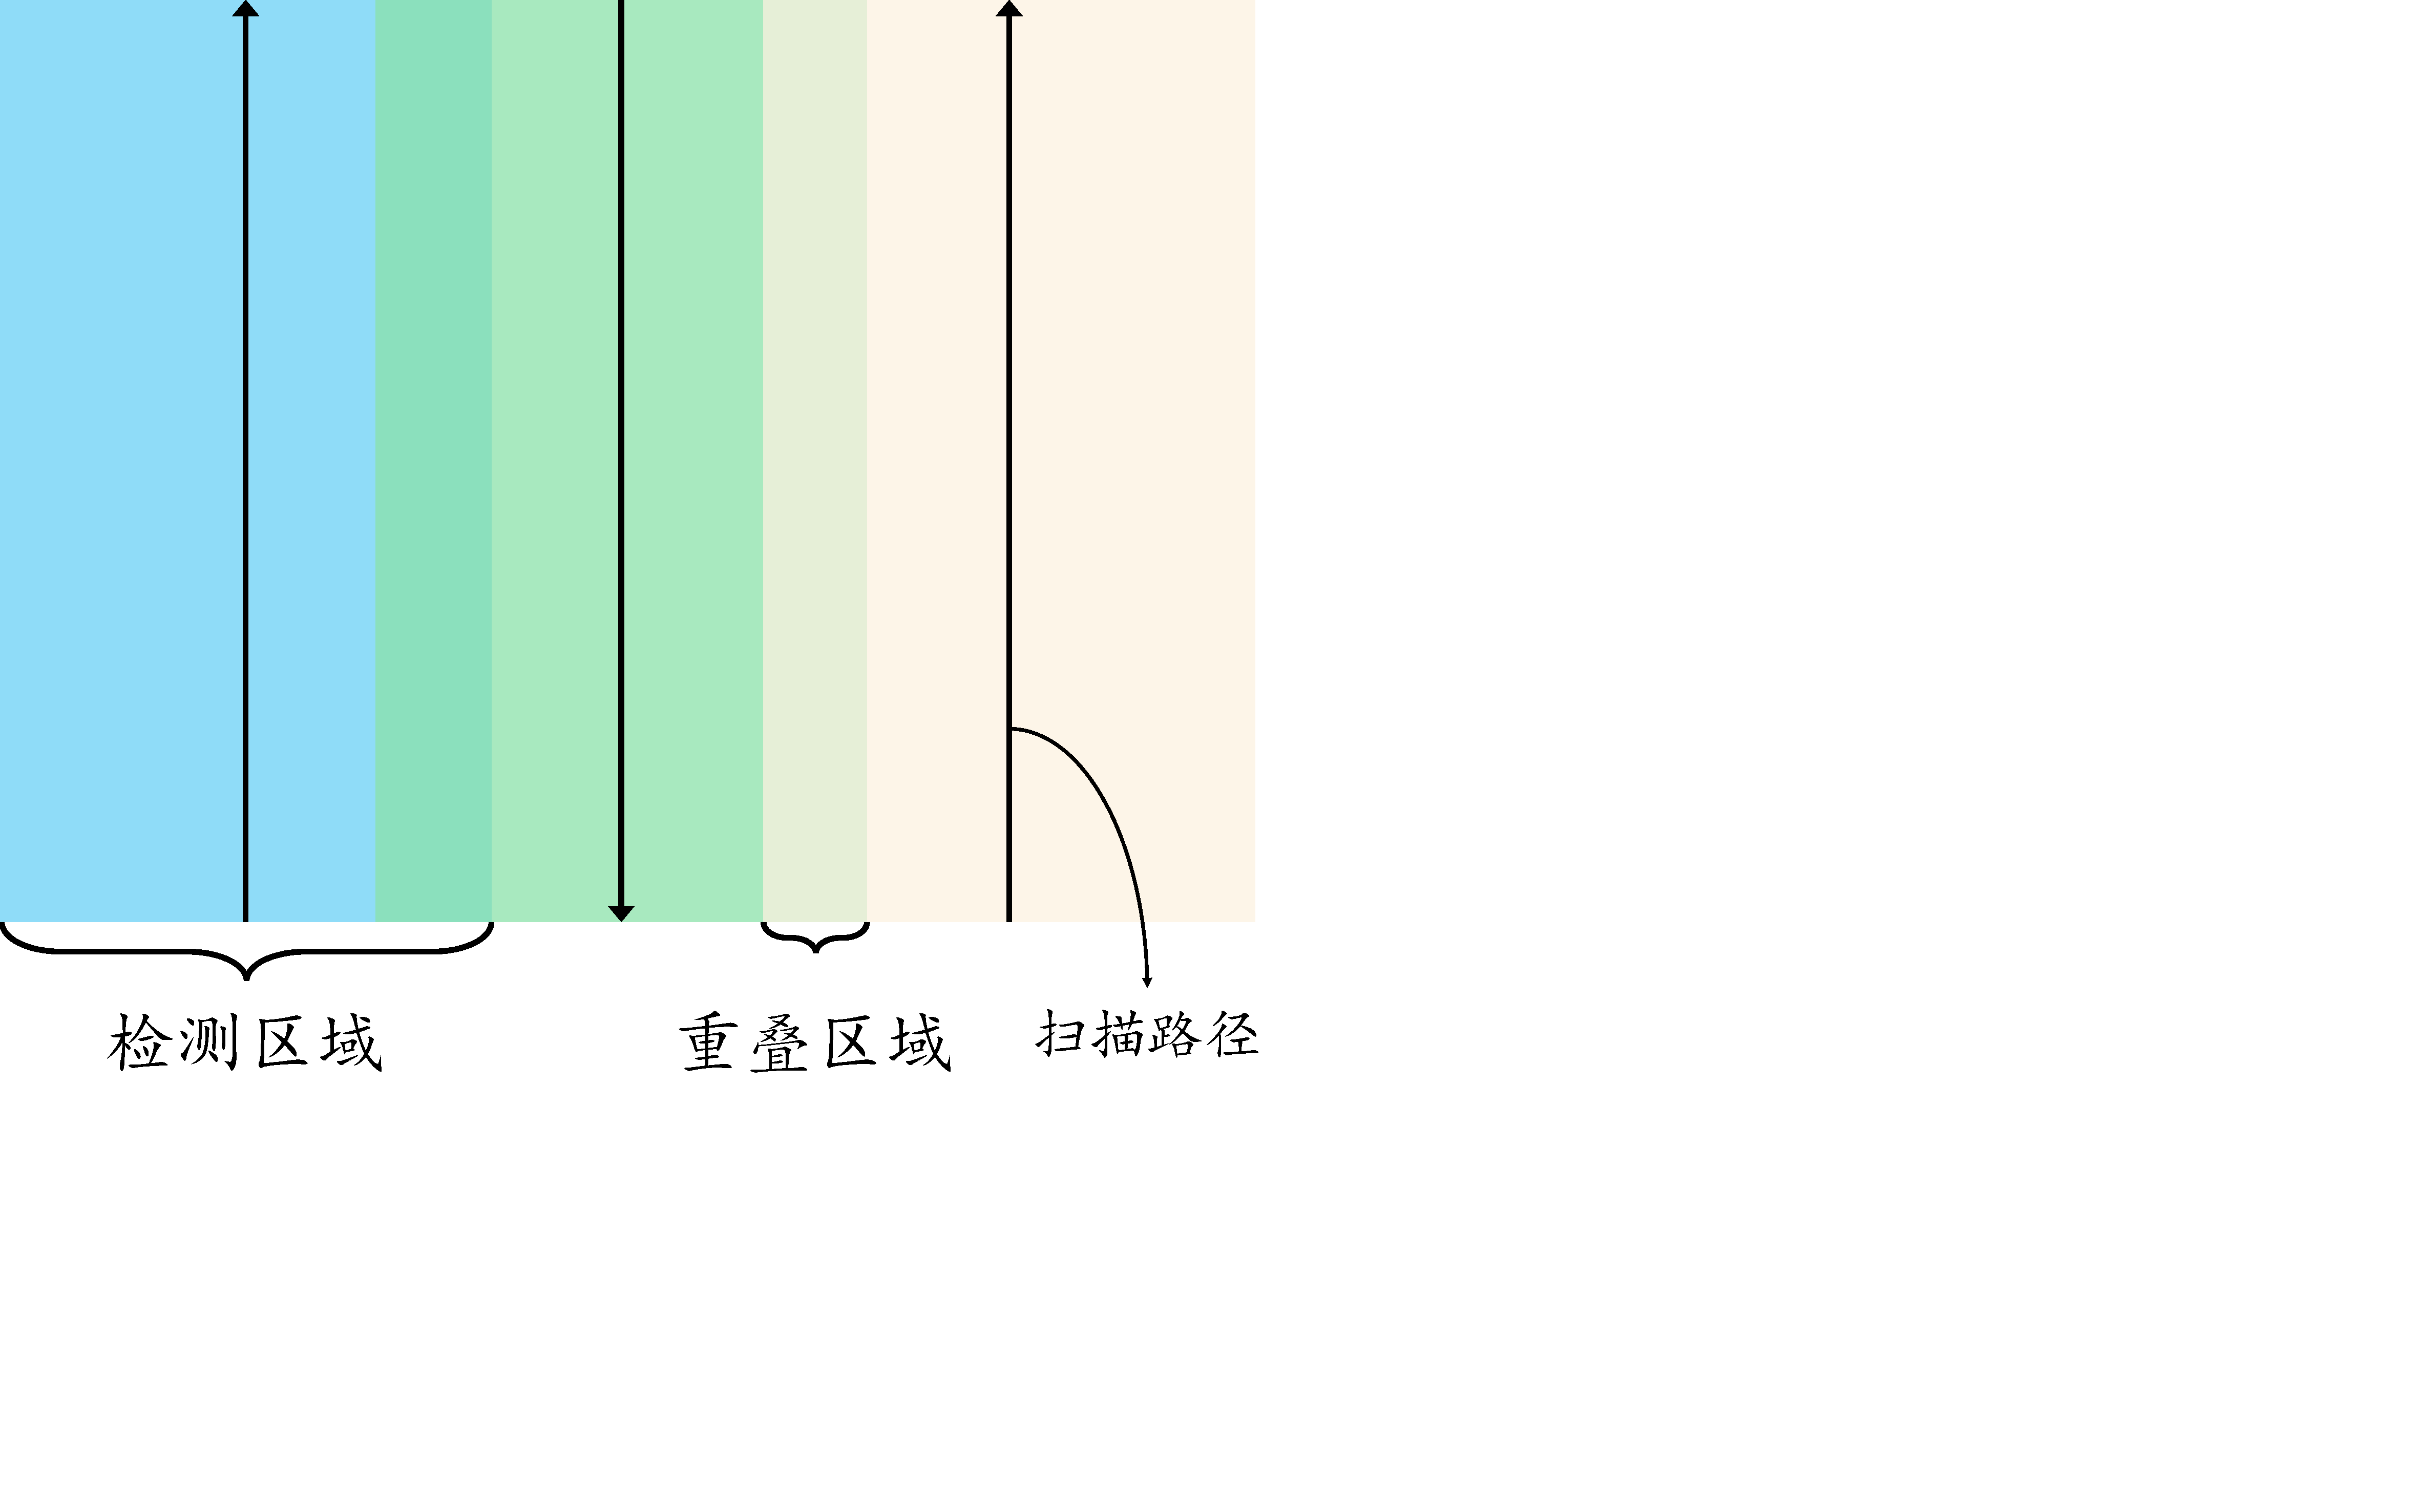
\includegraphics[width=0.4\textwidth,trim=0cm 14cm 35cm 0cm,clip]{figures/图3.pdf}}
		\hspace*{1cm}
		\subcaptionbox{覆盖宽度、路径间距和重叠率的关系\label{fig:图2b}}
		{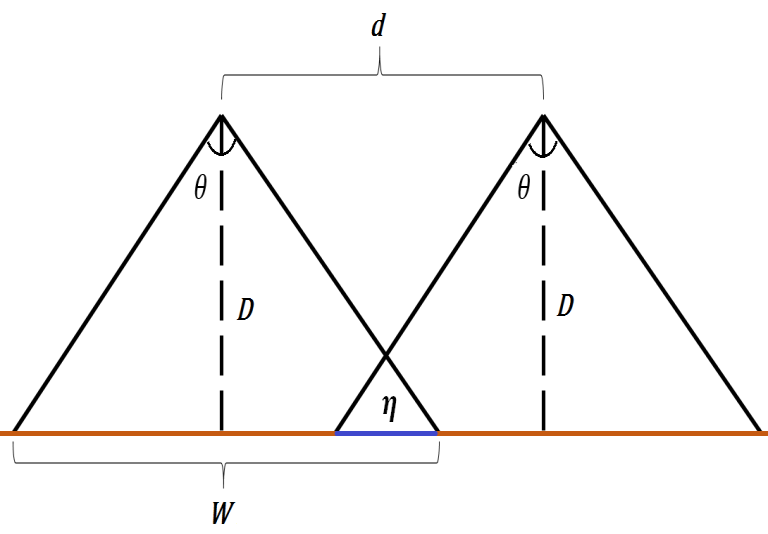
\includegraphics[width=0.5\textwidth,trim=0cm 0cm 0cm 0cm,clip]{figures/图4.png}}
		\caption{扫描条带及覆盖宽度示意图}
		\label{fig:条带对比}
	\end{figure}
	
	现对检测三棱柱形工件的斜面的平整度，对其斜面进行扫描，即摆放成横截面为三角形的样子，垂直于扫描方向的竖直平面与被测工件斜面的交线构成一条与水平面夹角为 \(\alpha\) 的斜线（图\ref{fig:图3}），称 \(\alpha\) 为斜面的倾角。
	
	\newpage
	\paragraph*{问题1} 请建立线激光测量的覆盖宽度及相邻扫描条带之间重叠率的数学模型。
	
	\begin{figure}[h!]
		\centering
		\vspace*{0pt}
		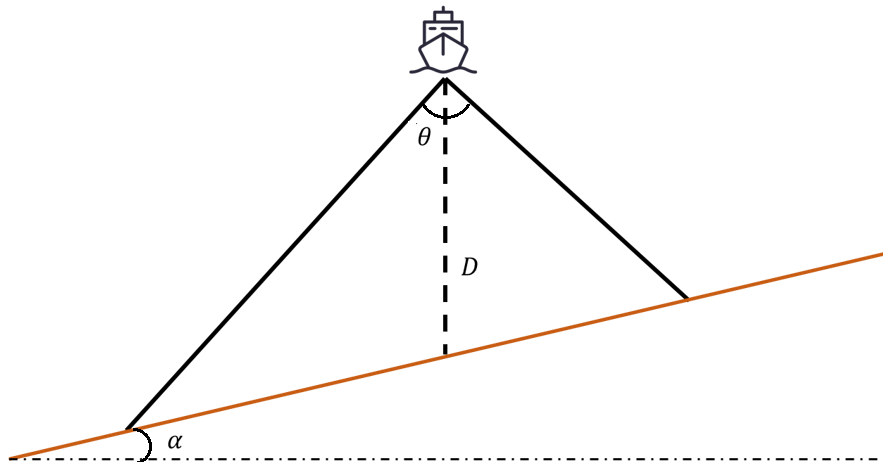
\includegraphics[width=0.6\textwidth,trim=0cm 0cm 0cm 1cm,clip]{figures/图7.png}
		\caption{问题1的示意图}
		\label{fig:图3}
	\end{figure}
	
	若激光发射张角为 \(120^{\circ}\)，工件斜面的倾角为 \(1.8^{\circ}\)，斜面中心点处的测量距离（传感器到工件表面的垂直距离）为 \(70 \mathrm{mm}\)，扫描路径间距 \(d = 100 \mathrm{mm}\)，利用上述模型计算表1中所列位置的指标值，将结果填入表1。
	
	\begin{table}[h!]
		\centering
		\caption{问题1的计算结果}
		\begin{tabular}{cccccc}
			\toprule
			测量点距中心点的距离/mm & -600 & -300 & 0 & 300 & 600 \\
			\midrule
			测量距离/mm & & & 70 & & \\
			覆盖宽度/mm & & & & & \\
			与前一条扫描条带的重叠率/\% & — & & & & \\
			\bottomrule
		\end{tabular}
	\end{table}
	
	\vspace*{-15pt}
	\paragraph*{问题2}
	
	考虑一个矩形待测斜面（图\ref{fig:图4}），扫描方向与斜面法向在水平面上投影的夹角为 \(\beta\)，请建立线激光测量覆盖宽度的数学模型。
	
	\begin{figure}[h!]
		\centering
		\vspace*{0pt}
		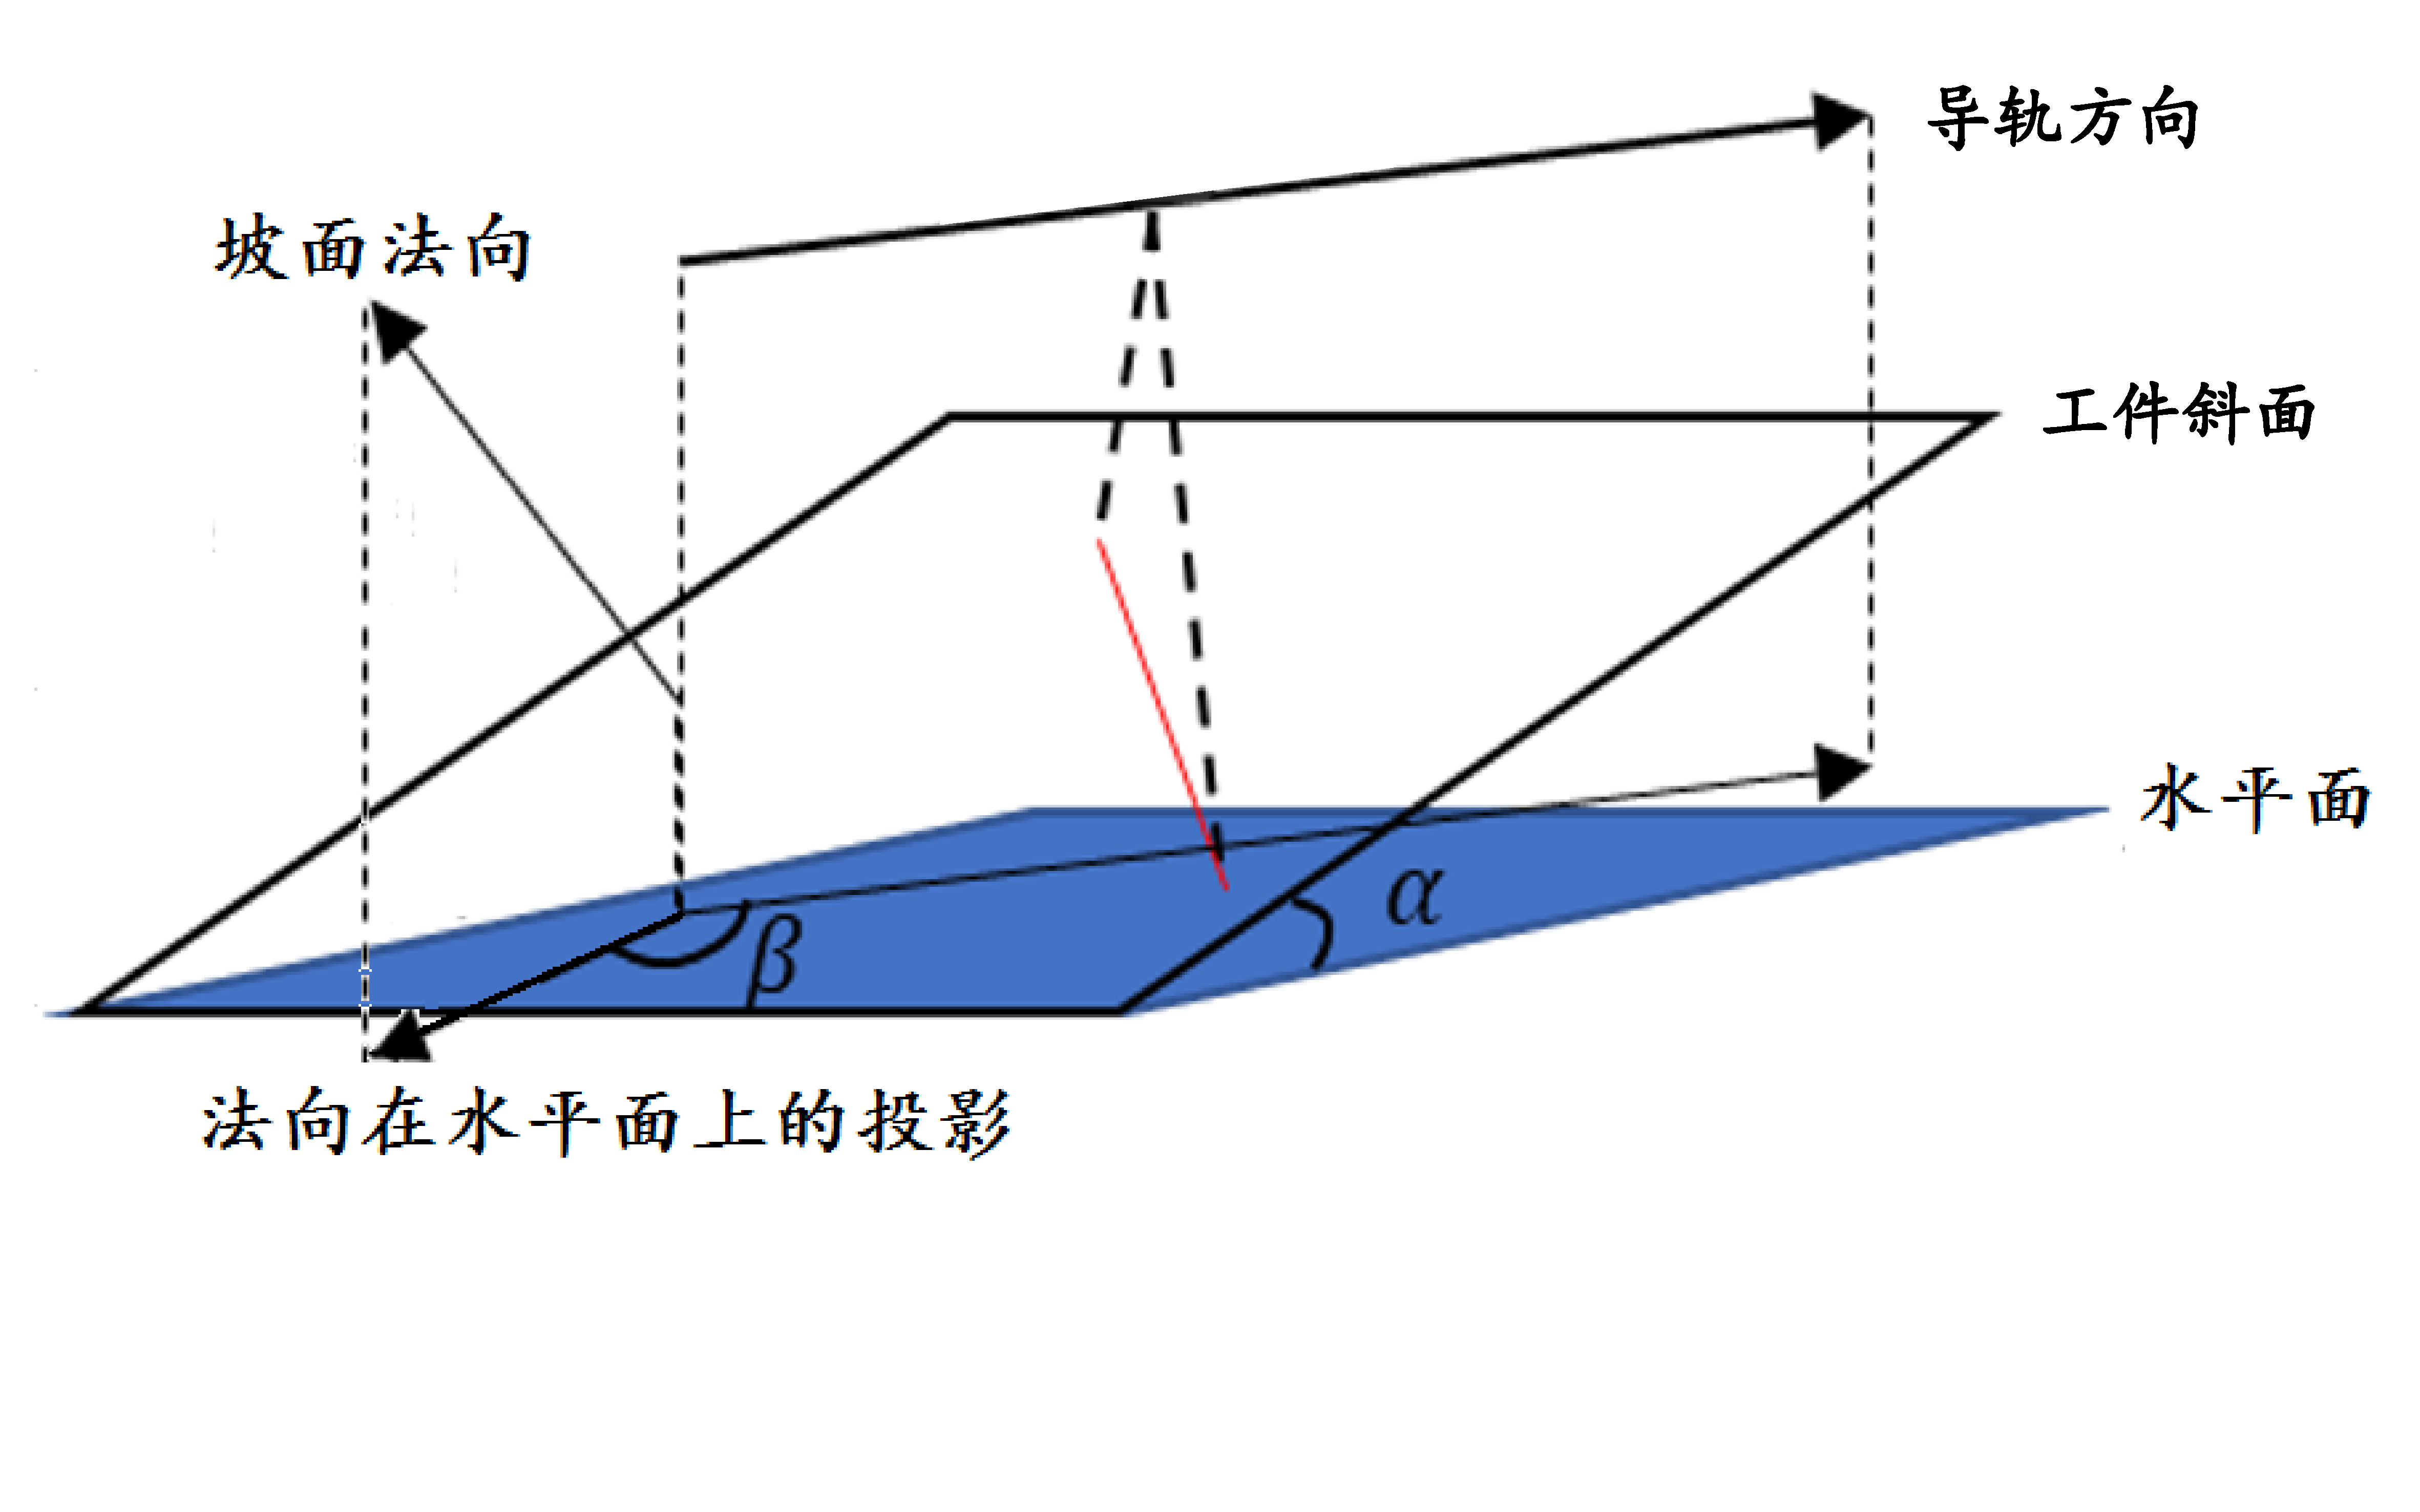
\includegraphics[width=0.6\textwidth,trim=0cm 11cm 0cm 0cm,clip]{figures/图8.pdf}
		\caption{问题2的示意图}
		\label{fig:图4}
	\end{figure}
	
	若激光发射张角为 \(120^{\circ}\)，斜面倾角为 \(1.8^{\circ}\)，斜面中心点处的测量距离为 \(120\mathrm{mm}\)，利用上述模型计算表2中所列位置线激光测量的覆盖宽度，将结果填入表2。
	
	\begin{table}[h!]
		\centering
		\caption{问题2的计算结果}
		\begin{tabular}{cccccc}
			\toprule
			\multirow{2}{*}{扫描方向夹角/°} & \multicolumn{5}{c}{传感器距中心点的距离/mm} \\
			\cmidrule(lr){2-6}
			& 0 & 50 & 100 & 150 & 200 \\
			\midrule
			0 & & & & & \\
			60 & & & & & \\
			120 & & & & & \\
			\bottomrule
		\end{tabular}
	\end{table}
	
	\newpage
	
	\begin{center}
		\section*{解答}
	\end{center}
	
	\subsection*{问题1解答}
	
	\subsubsection*{1. 建立坐标系}
	
	如图\ref{fig:图3}所示，建立空间直角坐标系。设扫描方向为\(y\)轴方向，与扫描方向垂直的水平方向为\(x\)轴方向，垂直方向为\(z\)轴（测量距离）方向。工件斜面与水平面的夹角为\(\alpha\)，倾角方向沿着\(x\)轴。设扫描路径经过斜面上的一点，该点处的测量距离为\(D_0\)。对于坐标为\((x, y)\)的斜面上的点，其测量距离\(D(x)\)可以表示为：
	\[
	D(x) = D_0 + x \tan \alpha
	\]
	
	\subsubsection*{2. 覆盖宽度的推导}
	
	激光发射张角为\(\theta\)。在平整表面情况下，覆盖宽度\(W\)与测量距离\(D\)的关系为：
	\[
	W = 2D \tan \frac{\theta}{2}
	\]
	
	在倾斜表面情况下，传感器正下方的测量距离为\(D_0\)。激光线在垂直于扫描方向的平面内，以张角\(\theta\)向两侧发射。由于工件表面是倾斜的，左右两侧的覆盖距离不再对称。
	
	设传感器位于原点\(O(0,0)\)，测量距离为\(D_0\)。左侧（\(x<0\)方向）表面的倾角导致测量距离变短，右侧（\(x>0\)方向）表面的倾角导致测量距离变长。
	
	左侧最远点\(x_L\)满足几何关系：
	\[
	\tan\left(\frac{\theta}{2}\right) = \frac{-x_L}{D(x_L)} = \frac{-x_L}{D_0 + x_L \tan \alpha}
	\]
	解出\(x_L\)：
	\[
	-x_L = (D_0 + x_L \tan \alpha) \tan\frac{\theta}{2}
	\]
	\[
	-x_L = D_0 \tan\frac{\theta}{2} + x_L \tan \alpha \tan\frac{\theta}{2}
	\]
	\[
	-x_L - x_L \tan \alpha \tan\frac{\theta}{2} = D_0 \tan\frac{\theta}{2}
	\]
	\[
	-x_L \left(1 + \tan \alpha \tan\frac{\theta}{2}\right) = D_0 \tan\frac{\theta}{2}
	\]
	\[
	x_L = -\frac{D_0 \tan\frac{\theta}{2}}{1 + \tan \alpha \tan\frac{\theta}{2}}
	\]
	
	右侧最远点\(x_R\)满足：
	\[
	\tan\left(\frac{\theta}{2}\right) = \frac{x_R}{D(x_R)} = \frac{x_R}{D_0 + x_R \tan \alpha}
	\]
	解出\(x_R\)：
	\[
	x_R = (D_0 + x_R \tan \alpha) \tan\frac{\theta}{2}
	\]
	\[
	x_R = D_0 \tan\frac{\theta}{2} + x_R \tan \alpha \tan\frac{\theta}{2}
	\]
	\[
	x_R - x_R \tan \alpha \tan\frac{\theta}{2} = D_0 \tan\frac{\theta}{2}
	\]
	\[
	x_R \left(1 - \tan \alpha \tan\frac{\theta}{2}\right) = D_0 \tan\frac{\theta}{2}
	\]
	\[
	x_R = \frac{D_0 \tan\frac{\theta}{2}}{1 - \tan \alpha \tan\frac{\theta}{2}}
	\]
	
	因此，覆盖宽度\(W\)为：
	\[
	W = x_R - x_L = D_0 \tan\frac{\theta}{2} \left( \frac{1}{1 - \tan \alpha \tan\frac{\theta}{2}} + \frac{1}{1 + \tan \alpha \tan\frac{\theta}{2}} \right)
	\]
	\[
	W = 2D_0 \tan\frac{\theta}{2} \cdot \frac{1}{1 - \left( \tan \alpha \tan\frac{\theta}{2} \right)^2}
	\]
	
	\subsubsection*{3. 重叠率的计算}
	
	设相邻两条扫描路径的间距为\(d\)，重叠率\(\eta\)定义为：
	\[
	\eta = 1 - \frac{d}{W}
	\]
	其中\(W\)取前一条扫描路径的覆盖宽度：
	\[
	\eta = 1 - \frac{d}{W_{\text{前}}}
	\]
	
	\subsubsection*{4. 计算结果}
	
	已知：\(\theta = 120^\circ\)，\(\alpha = 1.8^\circ\)，中心点测量距离\(D_0 = 70\) mm，扫描路径间距\(d = 100\) mm。
	
	计算\(\tan\frac{\theta}{2} = \tan 60^\circ = \sqrt{3} \approx 1.73205\)，\(\tan \alpha = \tan 1.8^\circ \approx 0.031426\)。
	
	首先计算中心点处（距离0 mm）的覆盖宽度：
	\[
	W_0 = 2 \times 70 \times 1.73205 \times \frac{1}{1 - (0.031426 \times 1.73205)^2} \approx 242.487 \times \frac{1}{1 - 0.002963} \approx 242.487 \times 1.00297 \approx 243.20 \text{ mm}
	\]
	
	对于距离中心点\(x\) mm处的测量点，该点的测量距离为\(D = D_0 + x \tan \alpha = 70 + x \times 0.031426\)。
	
	计算结果如下表：
	
	\begin{table}[h!]
		\centering
		\caption{问题1计算结果}
		\begin{tabular}{cccccc}
			\toprule
			测量点距中心点的距离/mm & -600 & -300 & 0 & 300 & 600 \\
			\midrule
			测量距离/mm & 51.14 & 60.57 & 70.00 & 79.43 & 88.86 \\
			覆盖宽度/mm & 177.62 & 210.41 & 243.20 & 275.98 & 308.77 \\
			与前一条扫描条带的重叠率/\% & — & 43.72 & 52.47 & 58.78 & 63.76 \\
			\bottomrule
		\end{tabular}
	\end{table}
	
	\subsection*{问题2解答}
	
	\subsubsection*{1. 数学模型}
	
	如图\ref{fig:图4}所示，设扫描方向与斜面法向在水平面上投影的夹角为\(\beta\)。此时，有效倾角变为扫描方向上的视倾角\(\alpha_{\text{eff}}\)：
	\[
	\tan \alpha_{\text{eff}} = \tan \alpha \cdot \cos \beta
	\]
	
	这是因为只有在垂直于扫描方向的方向上，斜面的倾角才会影响激光线的覆盖范围。\(\beta=0^\circ\)时，扫描方向与倾角方向垂直，有效倾角最大；\(\beta=90^\circ\)时，扫描方向与倾角方向平行，有效倾角为0。
	
	将\(\alpha\)替换为\(\alpha_{\text{eff}}\)，得到覆盖宽度的计算公式：
	\[
	W = 2D \tan\frac{\theta}{2} \cdot \frac{1}{1 - \left( \tan \alpha_{\text{eff}} \tan\frac{\theta}{2} \right)^2}
	\]
	
	\subsubsection*{2. 计算结果}
	
	已知：\(\theta = 120^\circ\)，\(\alpha = 1.8^\circ\)，中心点测量距离\(D_0 = 120\) mm。
	
	对于距离中心点\(L\) mm的测量点，该点的测量距离为\(D = D_0 + L \times \tan \alpha \cdot \cos \beta\)。
	
	计算结果如下表：
	
	\begin{table}[h!]
		\centering
		\caption{问题2计算结果}
		\begin{tabular}{cccccc}
			\toprule
			\multirow{2}{*}{扫描方向夹角/°} & \multicolumn{5}{c}{传感器距中心点的距离/mm} \\
			\cmidrule(lr){2-6}
			& 0 & 50 & 100 & 150 & 200 \\
			\midrule
			0 & 416.99 & 422.42 & 427.86 & 433.29 & 438.73 \\
			60 & 415.94 & 418.66 & 421.39 & 424.11 & 426.84 \\
			120 & 415.94 & 418.66 & 421.39 & 424.11 & 426.84 \\
			\bottomrule
		\end{tabular}
	\end{table}
	
\end{document}